\documentclass[sigconf,anonymous,review]{acmart}

%%
%% \BibTeX command to typeset BibTeX logo in the docs
\AtBeginDocument{%
  \providecommand\BibTeX{{%
    \normalfont B\kern-0.5em{\scshape i\kern-0.25em b}\kern-0.8em\TeX}}}

%% Rights management information.  This information is sent to you
%% when you complete the rights form.  These commands have SAMPLE
%% values in them; it is your responsibility as an author to replace
%% the commands and values with those provided to you when you
%% complete the rights form.
\setcopyright{acmcopyright}
\copyrightyear{2018}
\acmYear{2018}
\acmDOI{10.1145/1122445.1122456}

%% These commands are for a PROCEEDINGS abstract or paper.
\acmConference[Woodstock '18]{Woodstock '18: ACM Symposium on Neural
  Gaze Detection}{June 03--05, 2018}{Woodstock, NY}
\acmBooktitle{Woodstock '18: ACM Symposium on Neural Gaze Detection,
  June 03--05, 2018, Woodstock, NY}
\acmPrice{15.00}
\acmISBN{978-1-4503-XXXX-X/18/06}


\begin{document}

%%
%% The "title" command has an optional parameter,
%% allowing the author to define a "short title" to be used in page headers.
\title{Making Adversarial Fair Representation Learning Extinct with DINO}

%%
%% The "author" command and its associated commands are used to define
%% the authors and their affiliations.
%% Of note is the shared affiliation of the first two authors, and the
%% "authornote" and "authornotemark" commands
%% used to denote shared contribution to the research.
\author{Myles Bartlett}
\authornote{Both authors contributed equally to this research.}
\email{M.Bartlett@sussex.ac.uk}
\orcid{1234-5678-9012}
\author{Oliver Thomas}
\authornotemark[1]
\email{ot44@sussex.ac.uk}
\author{Thomas Kehrenberg}
\email{T.Kehrenberg@sussex.ac.uk}
\author{Novi Quadrianto}
\email{N.Quadrianto@sussex.ac.uk}
\affiliation{%
  \institution{Predictive Analytics Lab}
  \streetaddress{University of Sussex}
  \city{Falmer}
  \country{UK}
}
%%
%% By default, the full list of authors will be used in the page
%% headers. Often, this list is too long, and will overlap
%% other information printed in the page headers. This command allows
%% the author to define a more concise list
%% of authors' names for this purpose.
\renewcommand{\shortauthors}{Bartlett and Thomas, et al.}

%%
%% The abstract is a short summary of the work to be presented in the
%% article.
\begin{abstract}
There has been a plethora of papers about fairness in machine learning.
A promising approach is to pre-process the data in such a way that a broad range of semantic attributes are retained, but a specific set of \emph{protected} features are not.
Research in this area has predominantly applied adversarial methods to tabular data.
In the image domain, these approaches are less successful, with fairness constraints making a negligible impact on the efficacy of an auxiliary model.
We demonstrate empirically that using recent self-supervised methods can obtain results that are similar to, or exceed, those of adversarial approaches and provide a theoretical justification for our findings.
\end{abstract}

%%
%% The code below is generated by the tool at http://dl.acm.org/ccs.cfm.
%% Please copy and paste the code instead of the example below.
%%
\begin{CCSXML}
<ccs2012>
 <concept>
  <concept_id>10010520.10010553.10010562</concept_id>
  <concept_desc>Computer systems organization~Embedded systems</concept_desc>
  <concept_significance>500</concept_significance>
 </concept>
 <concept>
  <concept_id>10010520.10010575.10010755</concept_id>
  <concept_desc>Computer systems organization~Redundancy</concept_desc>
  <concept_significance>300</concept_significance>
 </concept>
 <concept>
  <concept_id>10010520.10010553.10010554</concept_id>
  <concept_desc>Computer systems organization~Robotics</concept_desc>
  <concept_significance>100</concept_significance>
 </concept>
 <concept>
  <concept_id>10003033.10003083.10003095</concept_id>
  <concept_desc>Networks~Network reliability</concept_desc>
  <concept_significance>100</concept_significance>
 </concept>
</ccs2012>
\end{CCSXML}

\ccsdesc[500]{Computer systems organization~Embedded systems}
\ccsdesc[300]{Computer systems organization~Redundancy}
\ccsdesc{Computer systems organization~Robotics}
\ccsdesc[100]{Networks~Network reliability}

%%
%% Keywords. The author(s) should pick words that accurately describe
%% the work being presented. Separate the keywords with commas.
\keywords{datasets, neural networks, gaze detection, text tagging}

%% A "teaser" image appears between the author and affiliation
%% information and the body of the document, and typically spans the
%% page.

\begin{teaserfigure}
    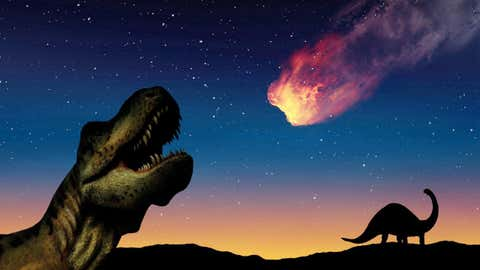
\includegraphics[width=\textwidth]{paper/assets/in-dinosaur killing comet.jpeg}
    \caption{Our title may be flippant, but we stand by dinosaurs being cool. On a serious note, this picture is of a meteorite descending rapidly to Earth, presumably about to cause the extinction event that led to the demise of the dinosaurs. This may be confusing because we are suggesting that self-supervised models (such as DINO) may make current approaches to censoring features obsolete. Following the analogy of this image, the dinosaur should be rapidly descending and a roaming herd of Adversarial Debiasing methods should be looking on with trepidation.}
    \label{fig:my_label}
\end{teaserfigure}

%%
%% This command processes the author and affiliation and title
%% information and builds the first part of the formatted document.
\maketitle


%-------------------------------------------------------------------------



\section{Introduction}
\label{sec:intro}
Computer Vision systems are being applied in increasingly consequential settings.
These systems excel in finding patterns in data, and in general we encourage them to exploit the simplest pattern possible.
A problem arises when there is a spurious pattern in the training data that isn't generally applicable.
For example, in a simple `cow or camel' classifier \citep{beery2018recognition}, all training images of cows are in luscious green pastures, and all camels are in brilliant desert sands.
At test time however, this may not be the case. 
A well-intending practitioner has inadvertently built a `green or yellow` classifier; a much simpler task that achieves excellent performance on the training set.

This is closely linked to the application-research areas of Domain Adaptation (DA), and Fairness in Machine Learning (FiML). 
In both cases there is a known variable that has manifested itself in the input domain in a way that is complex and non-trivial to remove.
In DA we may wish to make a representation of a road-scene independent of the weather so that an automated vehicle views a scene consistently regardless of sunshine or rain.
In FiML, we may wish to make a representation of a face-image independent of a race and gender so that a medical-analysis system works equally well for all ethnicity's and genders.
There is a subtle difference however: in DA the same scene can exist across multiple domains.
This is rarely the case though with inputs related to fairness.
In general, for Fairness problems the ``true'' mapping across domains is obscured from us.
This is why it is sometimes known as an \emph{aggravated} Domain Adaptation problem.

Recently, self-supervised models have been shown to be adept at ignoring features that are not of interest in the image.
Furthermore they produce excellent clustering of the data such that a simple $k$-Nearest-Neighbour model can produce competitive results \citep{caron2021emerging}.
We demonstrate that this these models are less easily-fooled by spurious patterns by focusing on the object of interest in an image, rather than low-level details.

\begin{itemize}
    \item Augmentations remove simple shortcuts. Forced to `look' at the object.
    \item Clustering more likely to be based on semantic attributes especially if performed on top of a representation learned via self-supervision \citep{van2020scan}.
    \item may need some sort of triplet loss so that e.g. long hair isn't closer to blonde and smiling.
\end{itemize}

\section{Background}
\label{sec:background}

\begin{itemize}
    \item Invariant Risk Minimisation
    \item Fair representations
    \item Adversarial methods
\end{itemize}

\balance % Needs to be placed int first column of the last page
\section{Experiments}
\label{sec:experiments}

\subsection{Datasets}
\label{sec:datasets}
To evaluate our hypothesis we use the following datasets.
\textbf{CelebA}. The \textbf{Celeb}rity \textbf{A}ttributes dataset contains $XXX,000$ images of celebrities.
In addition it contains $XX$ manually annotated features including hair colour, facial expression and gender.

\begin{itemize}
    \item CelebA
    \item NICO
    \item Waterbirds?
    \item GenFaces?
\end{itemize}

\subsection{Models}
\label{sec:models}

\begin{itemize}
    \item ERM
    \item IRM
    \item K\&C
    \item LAFTR?
    \item VFAE?
    \item DINO
\end{itemize}


\section{Conclusion}
\label{sec:conclusion}

We have shown that the emerging properties of self-supervised models are suitable for removing simple spurious correlations from images.
We propose that self-supervision may be more likely to produce fairer outcomes than adversarial approaches without requiring supervision.

\begin{acks}
To Robert, for the bagels and explaining CMYK and color spaces.
\end{acks}

\bibliographystyle{ACM-Reference-Format}
\bibliography{references}

\appendix
\section{Research Methods}


\end{document}
\endinput